

    %Abstract
    %Introduction (motivation for your work)
    %Background (literature review, or related work)
    %Methods (design and implementation)
    %Results and discussion  (include plots & figures, and detailed analysis in comparison to baseline and the literature, if applicable)
    %Conclusion

%\documentclass{article}
\documentclass[11pt,a4paper, twocolumn]{article}
%\usepackage[hyperref]{eacl2021}
\usepackage{times}
\usepackage{latexsym}
\usepackage{graphicx}
\renewcommand{\UrlFont}{\ttfamily\small}
\usepackage[nomarkers,nolists]{endfloat}

\usepackage{microtype}


\newcommand\BibTeX{B\textsc{ib}\TeX}

\title{Summarization for Social Media: Genre Specific}

\author{Trevor Johnson \\
  UC Berkeley  \\
  \texttt{trevorj@berkeley.edu} \\\And
  Andrew Beckerman \\
  UC Berkeley \\
  \texttt{abeckerman@berkeley.edu} \\}

\date{}

\begin{document}


\maketitle
\begin{abstract}

We present a method to produce abstractive summaries of informal social media text via neural abstractive summarization. We test models that have achieved state of the art text summarization performance in the news domain and evaluate their performance in the social media domain.
In addition, we test models trained on a specific genre against general models trained on all genres. We take this opportunity to show that [training and fine-tuning models on specific genres produces higher rouge scores].

\end{abstract}

\section{Introduction}

Text summarization is important for faster consumption of articles and text, saving time, and still providing the reader with the gist of an article. Figuring out what is ‘important’ in text summarization is challenging because the answer is highly dependent on the domain of the text, the target audience, and the goal of the summary itself.

Most summarization research is focused on new articles. However, as social media popularity increases, and in turn the generation of informal text, the need to summarize informal text will become more demanding.

With this in mind, we used the Webis-TLDR-17 corpus (Völske et al., 2017), a social media dataset, for our text summarization modeling. This dataset provides a summarization corpus from the domain of social media, consisting of 3 million reddit posts alongside so-called TL;DR summaries meaning "too long; didn't read".  These TL;DR summaries are written by social media posters writing long posts in anticipation of readers not having the patience to read an entire post. This gives us a text and summary written by the same person.

In addition, we wanted to explore the significance of understanding the genre of a post as it relates to model performance. We trained 4 separate models on 4 'genres' ('advice/story', 'gaming', 'media/lifestyle/sports' and 'other') and an overall model to evaluate whether a genre specific model can outperform a general model. To categorize the observations into different genres we used the subreddit \footnote{Subreddits are a forum dedicated to a specific topic on the website Reddit e.g., gaming, basketball, politics} of a post as a proxy for the 'genre' of the post. We feel the usefulness for understanding the importance of a genre could potentially extend beyond social media and be helpful in text summarization in many other domains including news articles.

We evaluate the model performance by using ROUGE metrics and manually evaluating the submissions.

[reference http://aclanthology.lst.uni-saarland.de/W17-4508.pdf]}

\begin{table}
\centering
\begin{tabular}{lrll}
\hline \textbf{Dataset} & \textbf{# docs (train/val/test} & \textbf{avg. post length} & \textbf{avg. summary legnth} \\ \hline
%\textbf{} & textbf{} & \multicolumn{words}{sentences} & \multicolumn{words}{sentences} \\
Overall & x & x & x \\
Advice/Story & 15,000/1,000/1,000 & x & x \\
Gaming & 15,000/1,000/1,000 & 4 & 15 \\
Media/Lifestyle/Sports & 15,000/1,000/1,000 & 4 & 15 \\
Other & 15,000/1,000/1,000 & 5 & 14 \\
\hline
\end{tabular}
\caption{\label{font-table} Comparison of summarization datasets with respect to overall corpus size, size of training, validation, and
test set, and average post and summary length (in terms of words and sentences)}
\end{table}

\begin{table}
\centering
\begin{tabular}{llllll}
\hline \textbf{Dataset} & \textbf{# docs (train/val/test} & \textbf{avg. post length} & \textbf{avg. summary legnth} \\ \hline
%\textbf{} & textbf{} & \multicolumn{words}{sentences} & \multicolumn{words}{sentences} \\
Overall & x & x & x \\
Advice/Story & 15,000/1,000/1,000 & x & x \\
Gaming & 15,000/1,000/1,000 & 4 & 15 \\
Media/Lifestyle/Sports & 15,000/1,000/1,000 & 4 & 15 \\
Other & 15,000/1,000/1,000 & 5 & 14 \\
\hline
\end{tabular}
\caption{\label{font-table} Comparison of summarization datasets with respect to overall corpus size, size of training, validation, and
test set, and average post and summary length (in terms of words and sentences)}
\end{table}

\section{Background}
\label{sec:length}

In 2018 a tldr challenge (Syed et al., 2018) was organized where participants submitted a model to do abstractive summarization on the same Webis-TLDR-17 corpus dataset. 5 submissions were evaluated. Models such as a fine-tuned BERT-based extractive, x, and x were submitted.

One of the metrics they used to evaluate the models was ROUGE. We include these models and respective ROUGE scores in this paper as a way to benchmark our own models performance.

No models were trained and tested on specific subreddits or genres.

%https://webis.de/downloads/publications/papers/syed_2019.pdf

\\

\section{Methods and Data}

\subsection{Exploratory Data Analysis}

Before modeling, we performed exploratory data analysis to understand the reddit data. 
The dataset consisted of 3.8 million observations, each containing the full reddit post, the "TLDR" or summary of the post, and the subreddit. 
We counted the number of words in each reddit post and summary by splitting on white space. 
The number of words in both the posts and summaries were heavily skewed right with average lengths of 278 and 27 respectively. 
While there were some posts and summaries with over 1,000 words, most had word counts in a reasonable range with 90\% of the posts containing between 42 and 795 words, and 90\% of the summaries containing between 3 and 75 words. 
Figure 1 shows histograms for the distribution of the distinct and total word counts for the reddit posts and summaries in our dataset. 


\begin{figure}
  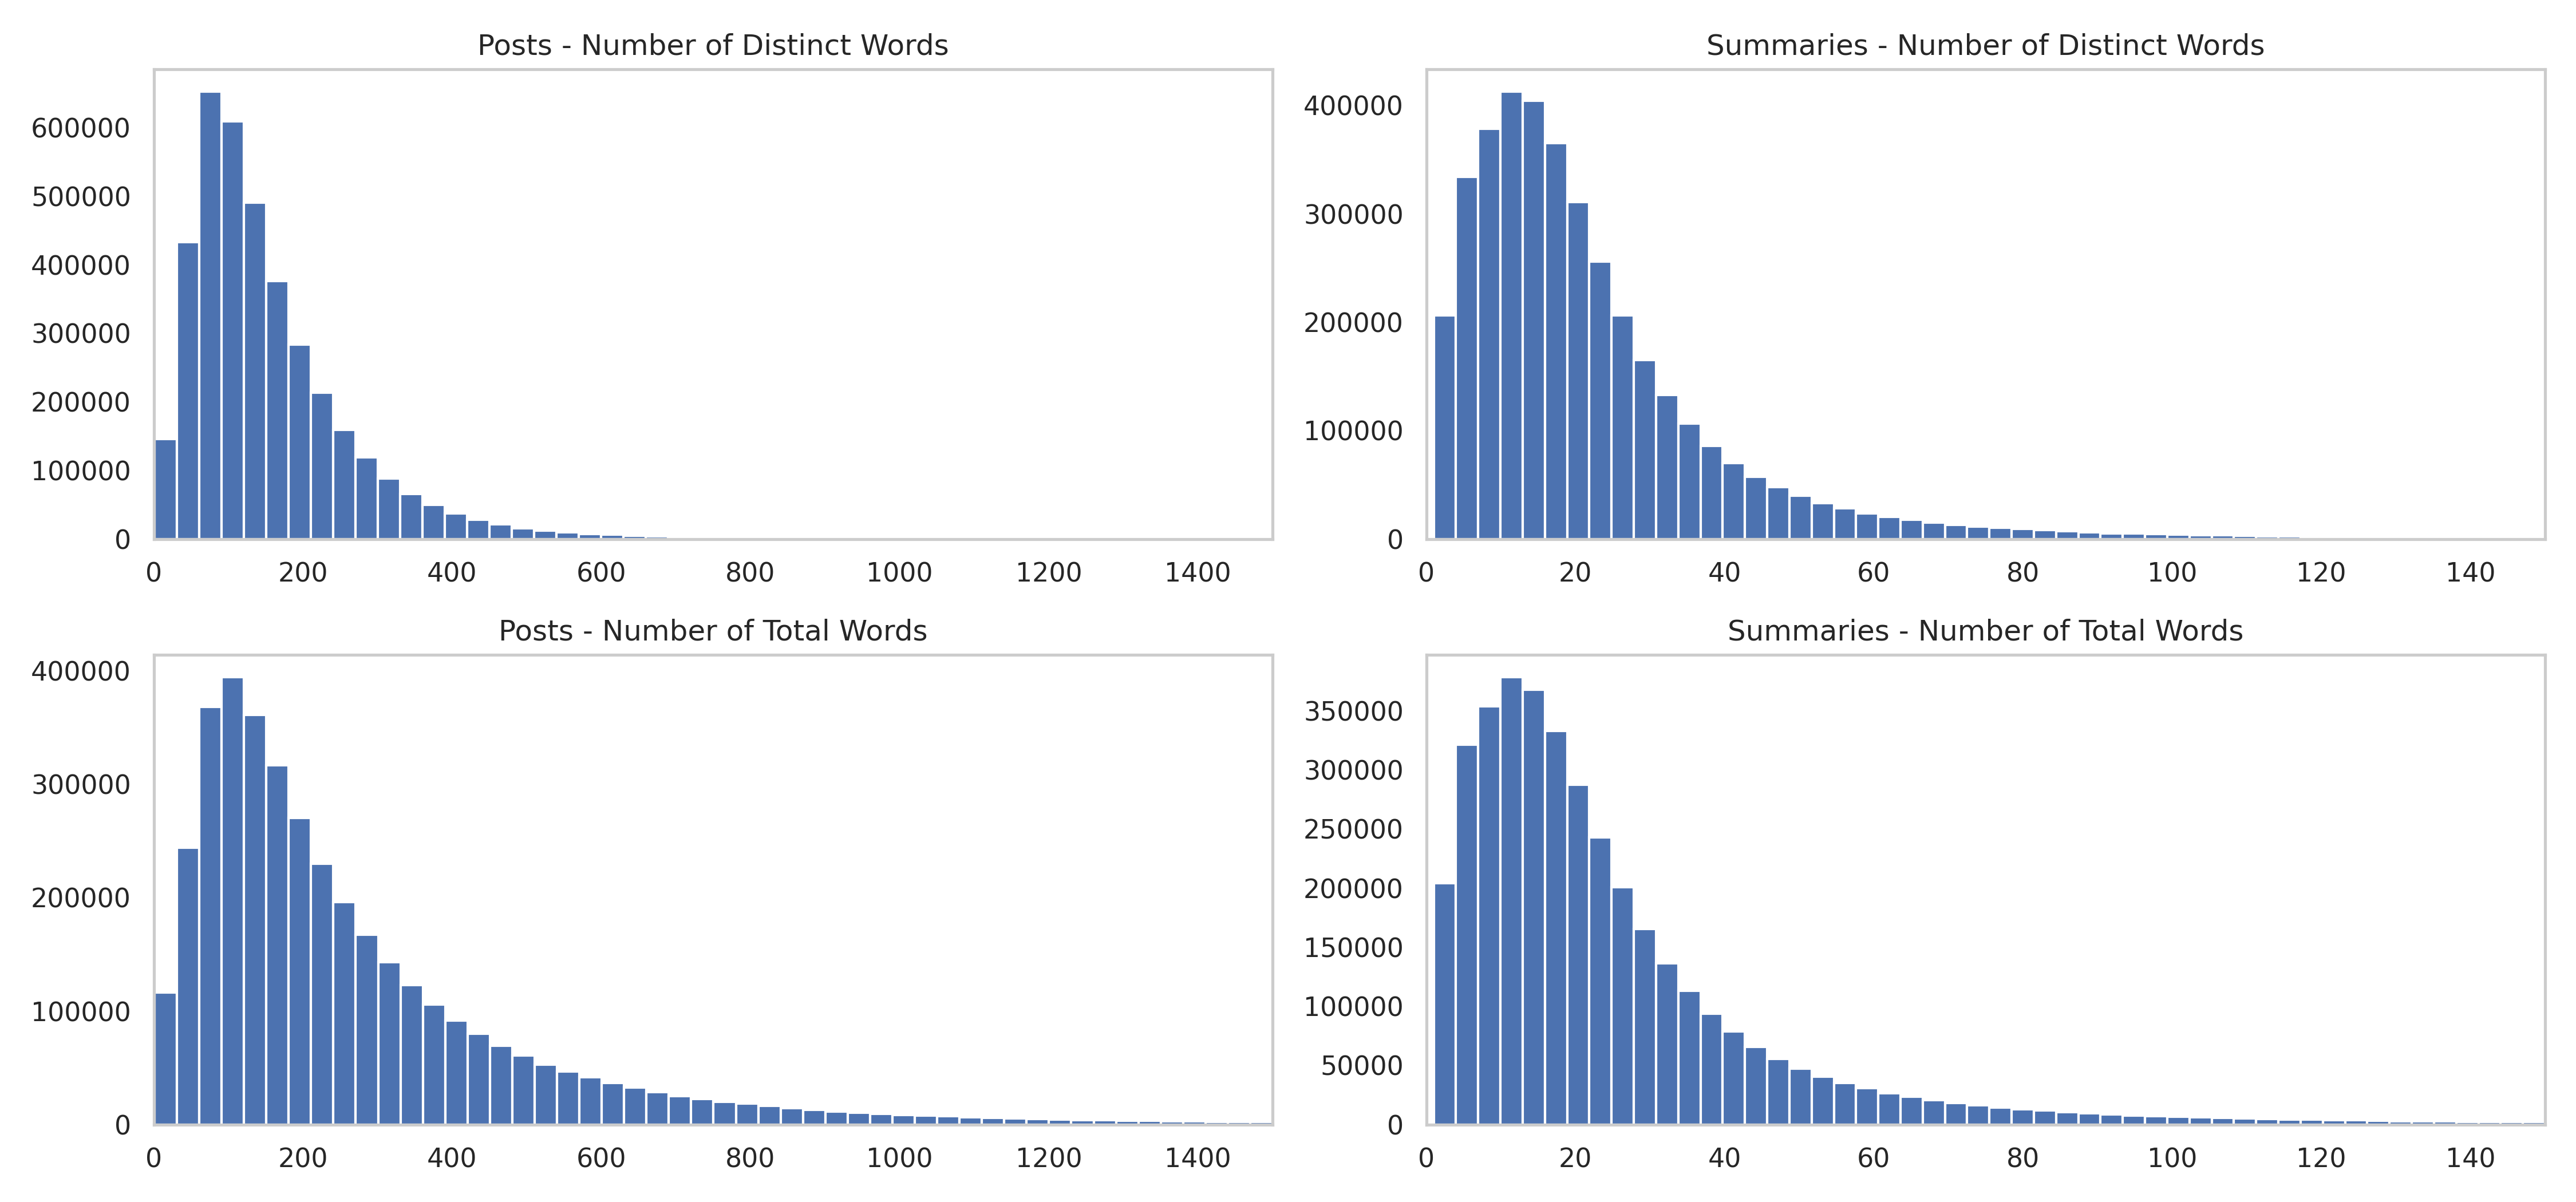
\includegraphics[width=\linewidth]{word_counts.png}
  \caption{Word count distributions}
  \label{fig:word_counts}
\end{figure}

\subsection{Subreddit Genres}

An initial investigation into the contents of the reddit posts and summaries showed that some contents nonsensically repeated the same word over and over, or would be extremely lengthy (over 3,000 words). With this in mind, we decided to filter down the dataset so it would only include reddit posts with word totals between 20 - 1000 and $\geq$ 10 unique words. In addition, each summary would only be between 2 - 100 total words and $\geq$ 2 unique words. With these filters in place, about 300,000 records were removed from our dataset. 

Next, we explored the many subreddits in our dataset as we hoped to use this information to create segmented NLP models. 
Because there were over 28,000 distinct subreddits in our dataset, it would be unreasonable to build separate NLP models for every distinct subreddit. 
Thus, we sought to group these subreddits into categories based on genre. 
We considered creating a separate NLP model or use unsupervised learning techniques to systematically cluster the subreddits into similar categories, 
but we ended up taking the time to group the subreddits into genres by hand and through regex keywords. 
In the end, we grouped the data into 4 distinct subreddit categories: gaming, advice/story, media/lifestyle/sports, and other. 
Several posts clearly overlapped with several different genres, but we felt this was a simple approach to create good enough separations to train different NLP models on. 
The counts for each subreddit genre can be found in figure 2. 

\begin{table}
  \centering
  \begin{tabular}{lrlll}
  \hline \textbf{Subreddit Genre} & \textbf{Post Count}\\ \hline
  Advice/Story & 1409813 \\
  Gaming & 501041 \\
  Media/Liftstyle/Sports & 455228 \\
  Other & 1184045 \\
  \hline
  \end{tabular}
  \caption{\label{font-table} Subreddit Genres}
\end{table}


\subsection{Modeling}

Sequence to sequence based transformer architectures have proven to achieve state of the art performance on the task of abstractive summarization (reference some paper in here: https://paperswithcode.com/task/text-summarization). 
Aghajanyan et al (cite this paper properly: https://arxiv.org/pdf/2008.03156v1.pdf) have achieved state of the art performance on a similar but smaller Reddit dataset with the challenge of abstractive summarization. 
This paper describes using a variation of the BART model to achieve state of the art performance of abstractive summarization on the Reddit TIFU subreddit. 
Seeing as BART has proven to achieve strong results for abstractive summarization on similar datasets, we decided to focus our efforts on using this model for our Reddit summarization task. 

After we began experimenting with training BART models on our dataset and generating summaries, we quickly realized the scale of our dataset would be a problem. 
We frequently ran out of memory, or would exhaust compute times at our disposal. 
Thus, we decided to downsample our large dataset to a more reasonable size for this project. 
From our cleaned dataset, we randomly sampled 17,000 observations from each of our 4 subreddit groups leaving us with a total of 68,000 observations for our analysis. 

Through initial BART model exploration, we decided to start with a BART model that was pretrained on both the XSUM and CNN/DM datasets. 
This pretrained model already generated fluent summaries on our dataset without fine tuning. 

We decied to compare generated summaries from the following three models and study their performances:
\begin{enumerate}
  \item Baseline: BART model pretrained on XSUM and CNN/DM without any fine tuning
  \item BART Full: BART model fine tuned on our entire Reddit dataset irrespective of subreddit
  \item BART Subreddit Split: Four separate BART models fine tuned on each of our four subreddit genre categories
\end{enumerate}


The input document was truncated to 1024 tokens and the length of the summary to 128 tokens. 

We used a BART model that was pre-trained on the XSUM and CNN data sets. We then fine-tuned the model on 60k posts and summaries and tested on 4k posts and summaries. In addition, we also trained 4 'genre-specific' BART models that were only trained on posts related to the genre for that specific model. 

We used ROUGE metrics to evaluate the model. We chose ROUGE because it is the most commonly used metic and we wanted to benchmark our model performance against models that were submitted from other papers. While evaluating the results from our model, we noticed that some summaries were not semantically accurate and we wanted to supplement our ROUGE metric with another metric to get a more a wholistic understanding of how our model was performing. In lieu of this, we decided to 'hand' grade x # of summaries and used these as the target summary to ensure the summaries were semantically accurate as well. 


FIGURE OF AN EXAMPLE POST SHOWING A SUMMARY NOT DOING A GIVING A GREAT SUMMARY


\section{Results and discussion}

\begin{table}
\centering
\begin{tabular}{lrlll}
\hline \textbf{Model} & \textbf{R-1} & \textbf{R-2} & \textbf{R-L} & \textbf{Gen Len} \\ \hline
BART & x & x & x & x \\
unified-pgn* & 19 & 4 & 15 & x \\
unified-vae-pgn* & 19 & 4 & 15 & x \\
transf-seq2seq* & 19 & 5 & 14 & x \\
pseudo-self-attn* & 18 & 4 & 13 & x \\
tldr-bottom-up* & 20 & 4  & 15 & x\\
\hline
\end{tabular}
\caption{\label{font-table} ROUGE-1,2, and L scores for the generated summaries and average word length}
\end{table}

\section{Conclusion}



\end{document}

